% Document class and parameters %
\documentclass[10pt,a4paper]{article}

% Document packages %
\usepackage{graphicx}
\usepackage{biblatex}
\usepackage{parskip}
\usepackage{listings}
\usepackage{caption}
\usepackage{subcaption}
\usepackage{amsmath}
\usepackage[most]{tcolorbox}


\graphicspath{{./Images/}}
\setlength{\parskip}{1em}

% Document Body %
\begin{document}
\begin{titlepage}
	\centering
	{\scshape\LARGE Imperial College London \par}
	\vspace{1cm}
	{\scshape\Large Mathematics: Year 2\par}
	\vspace{1.5cm}
	{\huge\bfseries Joint Distributed Random Variables \par}
	\vspace{2cm}
	{\Large\ Xin Wang }
	\vfill
	{\large \today\par}
\end{titlepage}

\begin{abstract}
Previous chapters have covered concepts to group data together in a coherent format such as
cumulative distribution function and probability density function. This chapter combines probability
and concepts like CDF and PDF.

Given random variables $X$ and $Y$ that are defined on a probability space, the joint probability
distribution for $X$ and $Y$ is a probability distribution that gives the probability in that each
of the random variables $X$ and $Y$ falls in any particular range or discrete set of specified values. 
\end{abstract}

\tableofcontents
\pagebreak

%%%%%%%%%%%%%%%%%%%%%%%%%%%%%%%%%%%%%%%%%%%%%%%%%%%%%%%%%%%%%%%%%%%%%%%%%%%%%%%%%%%%%%%%%%%%%%%%%%%%%%%%%%
% Sections Body %
\section{Introduction}

The previous chapter has only seen situations with single random variables but useful probability
statements often involve more than one random variable, usually pairs of random variables. For
example, in signal transmission, there will be a random variable $X$ to be the number of high-
quality signals received and the random variable $Y$ to be the number of low-quality signals
received - it is of interest the probabilities that can be expressed in terms of both $X$ and $Y$.

%%%%%%%%%%%%%%%%%%%%%%%%%%%%%%%%%%%%%%%%%%%%%%%%%%%%%%%%%%%%%%%%%%%%%%%%%%%%%%%%%%%%%%%%%%%%%%%%%%%%%%%%%%
\section{Two discrete random variables}
%%%%%%%%%%%%%%%%%%%%%%%%%%%%%%%%%%%%%%%%%%%%%%%%%%%%%%%%%%%%%%%%%%%%%%%%%%%%%%%%%%%%%%%%%%%%%%%%%%%%%%%%%%
\subsection{Joint probability distribution}

When dealing with \textbf{pairs} of random variables, the joint probability distribution is called
\textbf{bivariate distribution}. 

\textbf{Case Study}: In a new receiver transmitting digital information, each received bit is
classified as: Acceptable - \textit{Probability $0.9$}, Unacceptable - \textit{Probability $0.08$}
and Suspect - \textit{Probability $0.02$}. The ratings of each bit are \textbf{independent}. 

Four bits are transmitted. In the case study, the notations are defined as:
\begin{itemize}
    \item $X$ - Number of acceptable bits.
     
    The distribution of $X$ is \textbf{binomial} where $n = 4$ and $p = 0.9$.
    \item $Y$ - Number of suspect bits.
     
    The distribution of $X$ is \textbf{binomial} where $n = 4$ and $p = 0.08$.
\end{itemize}

The probabilities in a joint probability distribution is determined by the following example: Find
the probability that \textbf{two acceptable bits} and \textbf{one suspect bit} are received among
the four bits transmitted - $P(X=2, Y=1)$ - assuming the bits are independent of each other.
\begin{enumerate}
    \item Find the probability $P(aasu)$:
    \begin{align*}
        P(aasu) = 0.9 \times (0.9) \times (0.08) \times (0.02) = 0.0013
    \end{align*}
    \item Find the number of possible sequences with two $a$ and one $s$:
    \begin{align*}
        \frac{4!}{2!\times 1! \times 1!} = 12
    \end{align*}
    \item Find the joint probability:
    \begin{align*}
        P(aasu) = f_{XY}(2,1) = P(X=2,Y=1) = 12(0.0013) = 0.0156
    \end{align*}
\end{enumerate}

The following image describes the set of points $(x,y)$ in the range of $(X,Y)$ along with the
probability of each point within the \textbf{sample space} $S$.

\begin{figure} [h!]
    \centering
    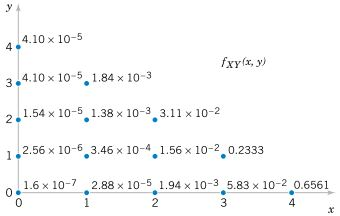
\includegraphics[]{Joint_case.JPG}
    \caption{Joint Probability Distribution of $X$ and $Y$}
    \label{fig:Case_joint}
\end{figure}

\begin{tcolorbox}[colback=white]
    \textbf{Joint probability distribution}: The probability distributions that defines how
    probability is assigned to all pairs of random variables $X$ and $Y$.
    $$
    F_{X,Y}(a,b) = P(X \leq a, Y \leq b) \; \text{where } -\infty < a \text{ and } b<\infty
    $$
\end{tcolorbox}

The joint probability distribution must satisfy the \textbf{characteristics of discrete
probability}:
\begin{enumerate}
    \item PMF must be non-negative.
    \item Sum of probabilities must be $1$.
\end{enumerate}

%%%%%%%%%%%%%%%%%%%%%%%%%%%%%%%%%%%%%%%%%%%%%%%%%%%%%%%%%%%%%%%%%%%%%%%%%%%%%%%%%%%%%%%%%%%%%%%%%%%%%%%%%%
\subsection{Marginal probability distributions (Marginal PMF)}

When more than one random variable is defined in a random experiment, it is important to
distinguish between the \textbf{joint probability distribution of $X$ and $Y$}, and the
\textbf{probability distribution of each individual variable}.

The \textbf{marginal probability distribution} of $X$ can be determined from the \textbf{joint
probability distribution} of $X$ by summing the joint PMF across the range of the other variable.

\textbf{Example 1}: Using the joint probability distribution of $X$ and $Y$ in Fig
\ref{fig:Case_joint}, find the marginal probability distribution of $X = 3$.
\begin{align*}
    P(X=3) &= P(X=3,\: Y=0) + P(X=3,\: Y=1) \\
    &= 0.0583 + 0.2333 \\
    &= 0.292
\end{align*}
Which is verified by:
\begin{align*}
    P(X=3) = {4 \choose 3}\times 0.9^3 \times 0.1^1 = 0.292
\end{align*}

\begin{tcolorbox}[breakable,colback=white]
\textbf{Marginal probability distribution} $(f_X(x))$: The individual probability distribution of a random
variable $X$.
\\
\begin{itemize}
    \item For random variable $X$: Summing probabilities in \textbf{each column}.
    $$
    f_X(x) = P(X=x) = \sum_{R_x}f_{XY}(x,\:y)
    $$
    where $R_x$ denotes the set of all points in the range of $(X,Y)$ for $X=x$.
    \\
    \item For random variable $Y$: Summing probabilities in \textbf{each row}.
    $$
    f_Y(y) = P(Y=y) = \sum_{R_y}f_{XY}(x,\:y)
    $$
    where $R_y$ denotes the set of all points in the range of $(X,Y)$ for $Y=y$. 
\end{itemize}
\end{tcolorbox}

%%%%%%%%%%%%%%%%%%%%%%%%%%%%%%%%%%%%%%%%%%%%%%%%%%%%%%%%%%%%%%%%%%%%%%%%%%%%%%%%%%%%%%%%%%%%%%%%%%%%%%%%%%
\section{Two continuous random variables}
%%%%%%%%%%%%%%%%%%%%%%%%%%%%%%%%%%%%%%%%%%%%%%%%%%%%%%%%%%%%%%%%%%%%%%%%%%%%%%%%%%%%%%%%%%%%%%%%%%%%%%%%%%
\subsection{Joint probability distribution}

The joint probability distribution of two continuous random variables is similar to the concept of
two discrete random variables. For example, consider injection modelling where the following
\textbf{continuous random variables} denote: $X$: The length of one dimension of an injection-molded
part and $Y$: the length of another dimension. The \textbf{sample space} of the random experiment consists of points in two dimensions.

Similar to the \textbf{probability density function} of \textbf{a single continuous random variable}, the
\textbf{joint probability density function} of \textbf{two continuous random variable} can be defined over
2-D space. 

The double integral of over a region $R$ provides the probability that $(X,Y)$ assumes a
value in $R$. This integral can be interpreted as the volume under the surface over the region $R$. 

\begin{figure} [h!]
    \centering
    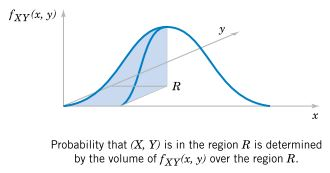
\includegraphics[scale=0.9]{Continu1.JPG}
    \caption{Joint probability density function for random variables $X$ and $Y$}
\end{figure}

\begin{tcolorbox}[breakable,colback=white]
    \textbf{Jointly continuous}: Two random variables X and Y are jointly continuous if there exists
    a nonnegative function $f_{XY}:\Re^2\rightarrow \Re$, such that, for any set $A\in \Re^2$:
    $$
    P\left[(X,Y)\in A\right] = \int \int_A f_{XY}(x,y)dx\: dy
    $$
    \\
    \textbf{Joint probability density function} $f_{XY}(x,y)$: A function that satifies the
    following:
    \begin{itemize}
        \item $f_{XY}(x,y)\geq 0$ for all $x,y$
        \item $\int_{-\infty}^\infty \int_{-\infty}^\infty f_{XY}(x,y)dx\: dy = 1$
        \item For any region $R$ of $2D$ space:
        $$
        P([X,Y]\in \Re) = \int_R \int f_{XY}(x,y)dx \: dy 
        $$
    \end{itemize}
\end{tcolorbox}

\textbf{Example 1}: Let the random variable $X$ denote the time until a computer server connects to your machine
(in milliseconds), and let $Y$ denote the time until the server authorizes you as a valid user (in
milliseconds). Each of these random variables measures the wait from a common starting time
and $X<Y$. 

Assume that the joint probability density function for X and Y:
$$
f_{XY}(x,y) = 6 \times 10^{-6} e^{(-0.001x - 0.002y)} \; \text{for } x<y
$$


If $X$ and $Y$ are continuous with a joint cumulative distribution function $F_{X,Y}(x,y)=P(X\leq x,
Y\leq y)$, the \textbf{joint probability density function} is defined as:
$$
    f_{X,Y}(x,y) = \frac{\partial^2 F_(X,Y)(x,y)}{\partial x \partial y}
$$
\begin{itemize}
    \item The region with nonzero probability is shaded. The property that this joint
    probability density function integrates to 1 can be verified by the integral of $f_{XY}(x, y)$ over this
    region.
    \begin{figure} [h!]
        \centering
        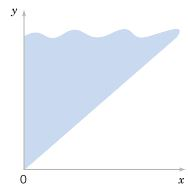
\includegraphics[scale=0.7]{Ex1.JPG}
        \caption{The joint probability density function of $X$ and $Y$ is non-zero over the shaded region}
    \end{figure}
    \begin{align*}
        \int_{-\infty}^\infty \int_{-\infty}^\infty f_{XY}(x,y)dy\: dx &= \int_0^\infty \left(\int_x^\infty 6 \times 10^{-6}e^{(-0.001x - 0.002y)dy}\right)dx \\
        &= 6 \times 10^{-6} \int_0^\infty \left(\int_x^\infty e^{-0.002x}dy\right)e^{-0.001x}dx \\
        &= 6 \times 10^{-6} \int_0^\infty \left(\frac{e^{-0.002y}}{0.002}\right)e^{-0.001x}dx \\
        &= 0.003\left(\int_0^\infty e^{-0.003x}dx\right) \\
        &= 0.003\left(\frac{1}{0.003}\right) = 1
    \end{align*}

    \item The probability that $X<1000$ and $Y<2000$ is determined as the integral over the darkly
    shaded region:
    \begin{figure} [h!]
        \centering
        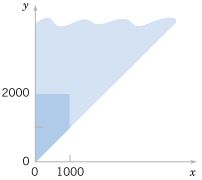
\includegraphics[scale=0.7]{Ex1a.JPG}
    \end{figure}
    \begin{align*}
        P(X\leq 1000, Y \leq 2000) &= \int_0^{1000} \int_x^{2000} f_{XY}(x,y) dy\:dx \\
        &= 6 \times 10^{-6} \int_0^{1000} \left(\int_x^{2000}e^{-0.002y}dy\right)e^{-0.001x} dx \\
        &= 6 \times 10^{-6} \int_0^{1000} \left(\frac{e^{-0.002x}-e^{-4}}{0.002}\right)e^{-0.001x}dx \\
        &= 0.003 \int_0^{1000} e^{-0.003x} - e^{-4}e^{-0.001x}dx \\
        &= 0.003 \left[\left(\frac{1-e^{-3}}{0.003}\right)-e^{-4}\left(\frac{1-e^{-1}}{0.001}\right)\right] \\
        &= 0.003(316.738 - 11.578) = 0.915
    \end{align*}
\end{itemize}

%%%%%%%%%%%%%%%%%%%%%%%%%%%%%%%%%%%%%%%%%%%%%%%%%%%%%%%%%%%%%%%%%%%%%%%%%%%%%%%%%%%%%%%%%%%%%%%%%%%%%%%%%%
\subsection{Marginal probability distributions (Marginal PMF)}

\begin{tcolorbox}[breakable,colback=white]
\textbf{The marginal probability density}: The probability distribution of random variables.
\\
\\
The marginal probability density functions of $X$ and $Y$, denoted by $f_X(x)$ and $f_Y(y)$ respectively, are obtained from the joint PDF:
\begin{align*}
    f_X(x) = \int_{-\infty}^{\infty} f_{X,Y}(x,y)dy \; \text{for } -\infty < x < \infty \\
    f_Y(y) = \int_{-\infty}^{\infty} f_{X,Y}(x,y)dx \; \text{for } -\infty < y < \infty 
\end{align*}
\end{tcolorbox}

As the marginal probability density describes the probability distribution of random variables, the
marginal density can be used to compute probabilities.

\textbf{Example 1}: Consider continuous random variables X and Y with joint PDF:
\begin{align*}
    f_{X,Y} (x,y) = 
    \begin{cases}
        \frac{6}{5}(x+y^2) & 0\leq x \leq 1, \; 0\leq y \leq 1 \\
        0 & \text{Otherwise}
    \end{cases}
\end{align*}
\begin{enumerate}
    \item Find $f_X(x)$:
    \begin{align*}
        f_X(x) &= \int_{-\infty}^\infty f_{X,Y}(x,y)dy \\
        &= \frac{6}{5}\int_0^1 (x+y^2) dy \\
        &= \frac{6}{5}\left[xy + \frac{y^3}{3}\right]_0^1 \\
        &= \frac{6}{5}x + \frac{2}{5}
    \end{align*}
    \item Find $f_Y(y)$:
    \begin{align*}
        f_X(x) &= \int_{-\infty}^\infty f_{X,Y}(x,y)dx \\
        &= \frac{6}{5}\int_0^1 (x+y^2) dx \\
        &= \frac{6}{5}\left[\frac{x^2}{2}+y^2x\right]_0^1 \\
        &= \frac{6}{5}y^2 + \frac{3}{5}
    \end{align*}
    \item Compute probability $P\left(\frac{1}{4}\leq Y \leq \frac{3}{4}\right)$ from the marginal probabilities:
    \begin{align*}
        P\left(\frac{1}{4}\leq Y \leq \frac{3}{4}\right) &= \int_{\frac{1}{4}}^{\frac{3}{4}} f_Y(y) dy \\
        &= \frac{37}{80} \\
        &\approx 0.4265
    \end{align*}
\end{enumerate}

If the region of integration \textbf{is not rectangular}, additional precautions need to be taken.

\textbf{Example 2}: Consider the continuous random variables X and Y with joint PDF given by:
\begin{align*}
    f_{X,Y}(x,y) = 
    \begin{cases}
        24xy & 0\leq x \leq 1, \; 0 \leq y \leq 1, \; x+y \leq 1 \\
        0 & \text{Otherwise}
    \end{cases}
\end{align*}
Note the extra constraint $y \leq 1-x$, resulting in the region of integration being:
\begin{figure} [h!]
    \centering
    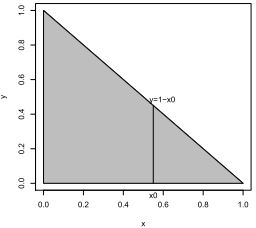
\includegraphics[scale=0.7]{Ex2_inter.JPG}
\end{figure}
\begin{enumerate}
    \item Establish that it is a \textbf{valid PDF} since the region is triangular:
    \begin{align*}
        \int_{-\infty}^{\infty} \int_{-\infty}^{\infty} f_{X,Y}(x,y) dxdy &= \int_0^1\left(\int_0^{1-x}24xy dy\right) dx \\
        \int_0^1 24x \left[\frac{y^2}{2}\right]_{y=0}^{y=1-x} dx \\
        &= \int_0^1 12x(1-x)^2 dx \\
        &= 1
    \end{align*}
    \item Obtain marginal distribution of $X$:
    \begin{align*}
        f_X(x) &= \int_{-\infty}^\infty f_{X,Y}(x,y) dy \\
        &= \int_0^{1-x}24xy dy \\
        &= 12x(1-x)^2
    \end{align*}
\end{enumerate}

%%%%%%%%%%%%%%%%%%%%%%%%%%%%%%%%%%%%%%%%%%%%%%%%%%%%%%%%%%%%%%%%%%%%%%%%%%%%%%%%%%%%%%%%%%%%%%%%%%%%%%%%%%
\subsection{Independence}

The definition of independence for continuous random variables is similar to the definition for
discrete random variables i.e.  If $f_{XY}(x, y) = f_X(x) f_Y(y)$ for all $x$ and $y$, $X$ and $Y$
are \textbf{independent}.

\begin{tcolorbox}[breakable,colback=white]
    For continuous random variables X and Y are said to be \textbf{independent}, if it satisfies the
    following:
    \begin{enumerate}
        \item $f_{XY}(x, y) = f_X(x) f_Y(y)$ for all x and y.
        \item $f_{Y|x}(y) = f_Y(y)$ for all $x$ and $y$ with $f_X(x)>0$
        \item $f_{X|y}(x) = f_X(x)$ for all $x$ and $y$ with $f_Y(y)>0$
        \item $P(X \leq x \cap Y \leq y) = P(X \leq x)P(Y \leq y)$
    \end{enumerate}
\end{tcolorbox}

Random variables are \textbf{independent} if the joint PMF or PDF can be expressed as a \textbf{product} of the
marginal PMF or PDF.

\textbf{Example 1}: Given the following discrete random variables, determine if $X$ and $Y$ are dependent. 
\begin{figure} [h!]
    \centering
    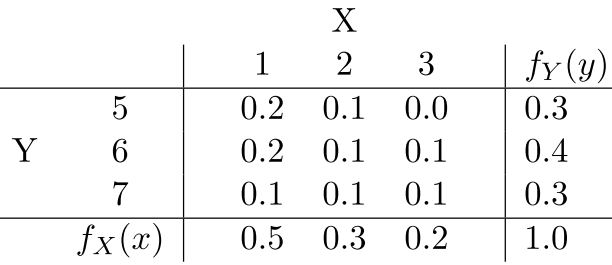
\includegraphics[scale=0.5]{Table.JPG}
\end{figure}
\begin{enumerate}
    \item Calculate the product of any marginal PDF: 
    \begin{align*}
        f_X(1) \times f_Y(7) = 0.5 \times 0.3 = 0.15 
    \end{align*}
    \item Calculate the joint PDF:
    \begin{align*}
        f_{X,Y}(1,7) = 0.1
    \end{align*}
    \item Conclude: $X$ and $Y$ are dependent.
    \begin{align*}
        f_X(1) \times f_Y(7) \neq f_{X,Y}(1,7)
    \end{align*}
\end{enumerate}

%%%%%%%%%%%%%%%%%%%%%%%%%%%%%%%%%%%%%%%%%%%%%%%%%%%%%%%%%%%%%%%%%%%%%%%%%%%%%%%%%%%%%%%%%%%%%%%%%%%%%%%%%%
\subsection{More than 2 variables}

The \textbf{joint PDF and CDF} are defined similarly to the previous concept:
\begin{itemize}
    \item \textbf{Joint CDF}:
    $$
        F_{X_1,X_2,\dots,X_n}(x_1, x_2,\dots,x_n) = P(X_1\leq x_1, X_2\leq x_2,\dots,X_n\leq x_n)
    $$
    \item \textbf{Joint PDF}:
    $$
        f_{X_1,X_2,\dots,X_n}(x_1, x_2,\dots,x_n) = \frac{\partial^n F_{X_1,X_2,\dots,X_n}(x_1, x_2,\dots,x_n)}{\partial x_1, \partial x_2, \dots, \partial x_n}
    $$
\end{itemize} 

\begin{tcolorbox}[breakable,colback=white]
\textbf{Mutual independence}: Every subset of variables are independent i.e. the joint PMF can be
expressed as a product of appropriate marginals (similar to previous chapter).
\begin{align*}
    F_{X_1,X_2,\dots,X_n}(x_1, x_2,\dots,x_n) = F_{X_1}(x_1)F_{X_2}(x_2)\dots F_{X_n}(x_n) \\
    f_{X_1,X_2,\dots,X_n}(x_1, x_2,\dots,x_n) = f_{X_1}(x_1)f_{X_2}(x_2)\dots f_{X_n}(x_n)
\end{align*}
\end{tcolorbox}

%%%%%%%%%%%%%%%%%%%%%%%%%%%%%%%%%%%%%%%%%%%%%%%%%%%%%%%%%%%%%%%%%%%%%%%%%%%%%%%%%%%%%%%%%%%%%%%%%%%%%%%%%%
\subsection{Conditional distributions}

Analogous to discrete random variables, we can define the \textbf{conditional probability distribution}
of $Y$ given $X=x$. This examines how one random variable behaves when a condition is placed on the
other random variable.

\begin{tcolorbox}[breakable,colback=white]
For random variables (\textbf{discrete} or \textbf{continuous}) $X$ and $Y$ with:
\begin{itemize}
    \item PMF (discrete) or PDF (continuous) denoted $f_{X,Y}(x,y)$
    \item Marginals denoted $f_X(x)$ and $f_Y(y)$
\end{itemize}
the \textbf{conditional PMF/PDF of $Y$ given $X=x$}:
$$
    f_{Y|X}(y|x) = \frac{f_{X,Y}(x,y)}{f_X(x)} \; \text{where } f_X(x) > 0
$$
\end{tcolorbox}

Since the function $f_{Y|x}(x)$ finds the probabilities of the all possible values for $Y$ given
that $X=x$, $f_{Y|x}(x)$ is a PDF for continuous random variables and a PMF for discrete random
variables. It has the following properties:
\begin{itemize}
    \item $f_{Y|x}(y) \geq 0$
    \item $\int_{R_x}f_{Y|x}(y)\; dy = 1$
    \item $P(Y\in B | X=x) = \int_B f_{Y|x}(y)\; dy$
\end{itemize}

\textbf{Example 1}: Consider the continuous random variables $X$ and $Y$ with joint PDF:
$$
    f_{X,Y}(x,y) = 
    \begin{cases}
        \frac{6}{5}(x+y^2) & 0 \leq x \leq 1, 0 \leq y \leq 1 \\
        0 & \text{Otherwise}
    \end{cases}
$$
find the PDF of $X$ given $Y=0.3$:
\begin{align*}
    f_{X|Y}(x|0.3) &= \frac{f(x,0.3)}{f_Y(0.3)} \\
    &= \frac{\frac{6}{5}(x+0.3^2)}{\frac{6}{5}(0.3)^2+\frac{3}{5}} \\
    &= \frac{100}{59}(x+0.3) \; \text{for } 0 \leq x \leq 1
\end{align*}

%%%%%%%%%%%%%%%%%%%%%%%%%%%%%%%%%%%%%%%%%%%%%%%%%%%%%%%%%%%%%%%%%%%%%%%%%%%%%%%%%%%%%%%%%%%%%%%%%%%%%%%%%%
\section{Expectation and Variance}
%%%%%%%%%%%%%%%%%%%%%%%%%%%%%%%%%%%%%%%%%%%%%%%%%%%%%%%%%%%%%%%%%%%%%%%%%%%%%%%%%%%%%%%%%%%%%%%%%%%%%%%%%%
\subsection{Expectation}
The \textbf{mean}, \textbf{expected value}, or \textbf{expectation} $E(X)$ of a random variable $X$ is a weighted average of the possible values that $X$ can
take, each value being weighted according to the probability of that event occurring i.e. the
long-term average of the random variable. 

Imagine observing many thousands of independent random values from the random variable of interest.
Take the average of these random values. The expectation is the value of this average as the sample size tends to infinity.

The result for the expected value of a function of a random variable extends to joint distributions
by weighting the PDF or PMF appropriately.

\begin{tcolorbox}[breakable,colback=white]
    For random variables $X$ and $Y$, the expected value of $g(X,Y)$ is:
    \begin{align*}
        E[X] = \mu_x = 
        \begin{cases}
            \sum_x\sum_y xf_{X,Y}(x,y) & $X$ \text{ and } $Y$ \text{ are discrete} \\
            \int_{-\infty}^{\infty} \int_{-\infty}^{\infty} xf_{X,Y}(x,y)\: dx dy & $X$ \text{ and } $Y$ \text{ are continuous}
        \end{cases}
    \end{align*}
    and 
    \begin{align*}
        E[Y] = \mu_y = 
        \begin{cases}
            \sum_x\sum_y yf_{X,Y}(x,y) & $X$ \text{ and } $Y$ \text{ are discrete} \\
            \int_{-\infty}^{\infty} \int_{-\infty}^{\infty} yf_{X,Y}(x,y)\: dx dy & $X$ \text{ and } $Y$ \text{ are continuous}
        \end{cases}
    \end{align*}
\end{tcolorbox}

Properties of Expectation:
\begin{enumerate}
    \item $E(X+Y)=E(X)+E(Y)$ for any random variable $X$ and $Y$.
    \item $Var(X\pm Y) = Var(X) + Var(Y)$ if random variable $X$ and $Y$ are \textbf{uncorrelated}.
\end{enumerate}

\textbf{Example 1}: Consider the data table, compute $E[g(X,Y)]$ where $g(X,Y) = X + Y$.
\begin{figure} [h!]
    \centering
    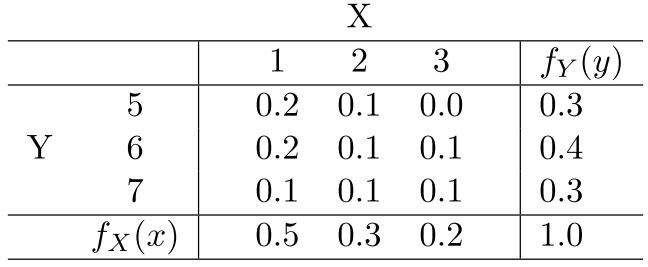
\includegraphics[scale=0.4]{Expect_ex1.JPG}
\end{figure}
\begin{align*}
    E[g(X,Y)] &= \sum_x \sum_y g(x,y) f_{X,Y}(x,y) \\
    &= 6(0.2)+7(0.2)+8(0.1) + \dots + 9(0.1) + 10(0.1) \\
    &= 7.7 
\end{align*}
%%%%%%%%%%%%%%%%%%%%%%%%%%%%%%%%%%%%%%%%%%%%%%%%%%%%%%%%%%%%%%%%%%%%%%%%%%%%%%%%%%%%%%%%%%%%%%%%%%%%%%%%%%
\subsubsection{Conditional expectation}

\begin{tcolorbox}[breakable,colback=white]
\textbf{Conditional expectation} of $X$ with respect to $Y$ $E[X|Y]$: The conditional expectation $g(y)$ of $X$ given that $Y=y$ is given by:
$$
    g(y) = E[X|Y = y] = 
    \begin{cases}
        \sum_i x_i P(X=x_i | Y=y) & \text{discrete} \\
        \int_{-\infty}^{+\infty} x f_{X|Y}(x|y)\: dx & \text{continuous}
    \end{cases}
$$
\end{tcolorbox}

Note that $E[X|Y=y]$ depends on the value of $y$ i.e. by changing $y$, $E[X|Y=y]$ can also change.
It is correct to say $E[X|Y=y]$ is a function of $y$:
$$
    g(y) = E[X|Y = y]
$$
It is also possible to think of $g(y)=E[X|Y=y]$ as a function of the value of random variable $Y$:
$$
    g(Y)=E[X|Y]
$$
Thus notation to indicate that $E[X|Y]$ is a random variable whose value equals $g(y)=E[X|Y=y]$ when
$Y=y$. If $Y$ is a random variable with range $R_Y={y_1,y_2,\dots}$, then $E[X|Y]$ is \textbf{also} a random
variable 

\textbf{Example 1}: Given the condition PDF of $X$ given that $Y=0.3$
$$
    f_{X|Y}(x|y) = \frac{100}{59}(x+0.3)
$$
find the \textbf{conditional expectation} of $X$ given that $Y=0.3$.
\begin{align*}
    E[X|Y = 0.3] &= \int_{-\infty}^\infty xf_{X|Y}(x|0.3)\: dx \\
    &= \left[\frac{100}{77}x^3 + \frac{9}{118}x^2 \right]_0^1 \\
    &= \frac{227}{354}
\end{align*}

\begin{tcolorbox}[breakable,colback=white]
    Common properties of conditional expectation:
    \begin{itemize}
        \item $E_Y[E[X|Y]] = E(X)$
        \item $E[ag(X)+h(X)|Y] = aE[g(X)|Y]+E[h(X)|Y]$
        \item $E[g(X)h(Y)|Y=y]=h(y)E[g(X)|Y=y]$
    \end{itemize}
\end{tcolorbox}

%%%%%%%%%%%%%%%%%%%%%%%%%%%%%%%%%%%%%%%%%%%%%%%%%%%%%%%%%%%%%%%%%%%%%%%%%%%%%%%%%%%%%%%%%%%%%%%%%%%%%%%%%%
\subsection{Conditional Variance}

Similar to the conditional expectation, the conditional variance of $X$ is defined as $Var(X|Y=y)$,
which is the variance of $X$ in the conditional space where $Y=y$.

\begin{tcolorbox}[breakable,colback=white]
For random variables $X$ and $Y$, the conditional variance $Var(X|Y)$ of $X$ with w.r.t $Y$ is the
random variable whose value at point $Y=y$ is defined by:
\begin{align*}
    Var[X|Y=y] = 
    \begin{cases}
        \sum_i [x_i - E[X|Y=y]]^2 P(X=x_i|Y=y) & \text{for discrete} \\
        \int_{-\infty}^{+\infty} [x - E[X|Y=y]]^2 f_{X|Y}(x|y)dx & \text{for continuous}
    \end{cases}
\end{align*}
\end{tcolorbox}

The \textbf{Law of Total Variance} states:
\begin{align*}
    Var(X)=E[Var(X|Y)]+Var(E[X|Y])
\end{align*}

%%%%%%%%%%%%%%%%%%%%%%%%%%%%%%%%%%%%%%%%%%%%%%%%%%%%%%%%%%%%%%%%%%%%%%%%%%%%%%%%%%%%%%%%%%%%%%%%%%%%%%%%%%
\section{Covariance and Correlation}

In probability theory and statistics, the concepts of \textbf{covariance} and \textbf{correlation} are
very similar and often used. Both the terms measure the relationship and the dependency between two
variables between dependent random variables $X$ and $Y$.

When comparing data samples from different populations:
\begin{itemize}
    \item \textbf{Covariance} measures the direction of the linear relationship between variables.
    \item \textbf{Correlation} measures both the strength and direction of the linear relationship between two variables.
\end{itemize}

Correlation is a function of the covariance. What sets them apart is the fact that correlation values are standardized whereas, covariance values are not. 

%%%%%%%%%%%%%%%%%%%%%%%%%%%%%%%%%%%%%%%%%%%%%%%%%%%%%%%%%%%%%%%%%%%%%%%%%%%%%%%%%%%%%%%%%%%%%%%%%%%%%%%%%%
\subsection{Covariance}

Covariance is a measure used to determine how much two variables change in tandem, the direction of
the \textbf{linear relationship} between the two variables. It generalizes the concept of variance to
multiple random variables. Instead of measuring the fluctuation of a single random variable, the
covariance measures the
fluctuation of two variables with each other.

Recall that the variance is the mean squared deviation from the mean for a single random variable
$X$:
$$
Var(X)=E[(X-E[X])^2].
$$

\begin{tcolorbox}[breakable,colback=white]
   \textbf{Covariance} between random variables $X$ and $Y$: 
   \begin{align*}
        \text{Cov}(X,Y )= E[(X-E[X])(Y-E[Y])] \\
        \Rightarrow \text{Cov}(X, Y ) = E[(X - \mu_x)(Y - \mu_y)]
   \end{align*}
   thus 
   \begin{align*}
        \text{Cov}(X, Y ) = 
        \begin{cases}
            \sum_X \sum_Y (x - \mu_x)(y - \mu_y)f_{X,Y}(x,y) & \text{discrete} \\
            \int_{-\infty}^{\infty} \int_{-\infty}^{\infty} (x-\mu_x)(y-\mu_y) f_{X,Y}(x,y) dx\: dy & \text{continuous}
        \end{cases}
   \end{align*}
   where $\mu_x$ and $\mu_y$ are the expected value of $X$ and $Y$ respectively.
\end{tcolorbox}

Common properties of covariance:
\begin{itemize}
    \item $\text{Cov}(X, Y ) = \text{Cov}(Y, X)$
    \item $\text{Cov}(X, X) = Var(X)$
    \item $\text{Cov}(X, a) = 0$ for any constant $a$
    \item $\text{Cov}(aX + b, cY + d) = ac \text{Cov}(X, Y )$
\end{itemize}

\begin{tcolorbox}[breakable,colback=white]
    It is generally simpler to find the covariance by expanding the definition of covariance:
    \begin{align*}
        \text{Cov}(X,Y) &=  E[(X-E[X])(Y-E[Y])] \\
        &= E[XY-E[X]Y-XE[Y]+E[X]E[Y]] \\
        &= E(XY) - E(X)E(Y) 
    \end{align*}
\end{tcolorbox}

Interpreting the results:
\begin{itemize}
    \item $\text{Cov}(X,Y)>0$: Large values of $X$ tend to be associated with large values of $Y$
    i.e. \textbf{higher the covariance, the stronger the relationship}.
    \item $\text{Cov}(X,Y)<0$: Large values of $X$ tend to be association with small values of $Y$.
    \item $\text{Cov}(X,Y)=0$: No simple linear relationship between the variables.
\end{itemize}
\begin{figure} [h!]
    \centering
    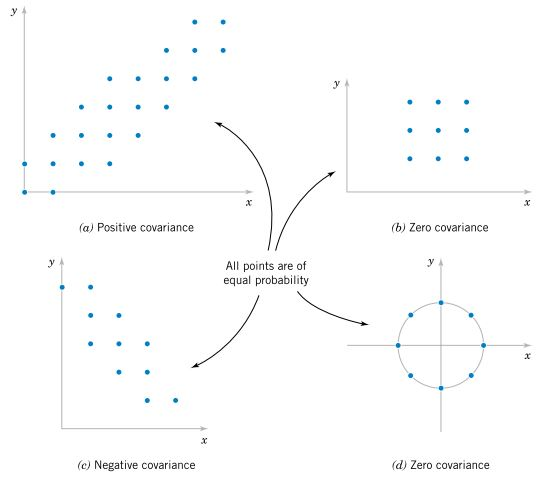
\includegraphics[scale=0.56]{covariance_type.JPG}
\end{figure}

\textbf{Example 1:} Consider discrete random variables $X$ and $Y$ with joint PMF:
\begin{align*}
    f_{X,Y}(x,y) = 
    \begin{cases}
        \frac{1}{2} & x=3, y=4 \\
        \frac{1}{3} & x=3, y=6 \\
        \frac{1}{6} & x=5, y=6 \\
        0 & \text{Otherwise}
    \end{cases}
\end{align*}
find the covariance:
\begin{enumerate}
    \item Find expected values $E(X)$ and $E(Y)$:
    \begin{align*}
        E(X) &= \frac{1}{2}(3) + \frac{1}{3}(3) + \frac{1}{6}(5) + 0 \\
        &= \frac{10}{3}
    \end{align*}\
    and 
    \begin{align*}
        E(Y) &= \frac{1}{2}(4) + \frac{1}{3}(6) + \frac{1}{6}(6) + 0 \\
        &= 5
    \end{align*}
    \item Find the $\text{Cov}(X,Y)$:
    \begin{align*}
        \text{Cov}(X,Y) &= E[(X-\mu_x)(Y-\mu_y)] \\
        &= \frac{\left(3-\frac{10}{3}\right)(4-5)}{2} + \frac{\left(3-\frac{10}{3}\right)(6-5)}{3} + \frac{\left(5-\frac{10}{3}\right)(6-5)}{6} + 0 \\
        &= \frac{1}{6} - \frac{1}{9} + \frac{5}{18} + 0 \\
        &= \frac{1}{3}
    \end{align*}
\end{enumerate}

\textbf{Example 2}: Recall the example with $X$ and $Y$ continuous, with joint PDF:
$$
f_{X,Y}(x,y) = 24xy
$$
for $0 \leq x \leq 1$, $0 \leq y \leq 1$, $ x + y \leq 1$, and $0$ otherwise.

Find the covariance.
\begin{enumerate}
    \item Find expect value $\mu_x$:
    \begin{align*}
        \mu_x &= \int_{-\infty}^{\infty} \int_{-\infty}^{\infty} x f_{X,Y}(x,y) \: dy \: dx \\
        &= \int_0^1 \int_0^{1-x} x 24xy \: dy\: dx \\
        &= \int_0^1 24x^2 \left[\frac{y^2}{2}\right]_0^{1-x} dx \\
        &= \int_0^1 (12x^2 - 24x^3 + 12x^4)dx \\
        &= \frac{2}{5}
    \end{align*}
    \item Find expect value $\mu_y$:
    \begin{align*}
        \mu_y &= \int_{-\infty}^{\infty} \int_{-\infty}^{\infty} y f_{X,Y}(x,y) \: dy \: dx \\
        &= \int_0^1 \int_0^{1-x} y 24xy \: dy\: dx \\
        &= \int_0^1 24x \left[\frac{y^3}{3}\right]_0^{1-x} dx \\
        &= \int_0^1 (8x - 24x^2 + 24x^3 - 8x^4)dx \\
        &= \frac{2}{5}
    \end{align*}
    \item Find the expect value $\mu_{xy}$:
    \begin{align*}
        \mu_{xy} &= \int_{-\infty}^{\infty} \int_{-\infty}^{\infty} xy f_{X,Y}(x,y)\: dy\:dx \\
        &= \int_0^1 \int_0^{1-x} xy 24 xy \: dy\:dx \\
        &= 8 \int_0^1 x^2 (1-x)^3 dx \\
        &= \frac{2}{15}
    \end{align*}
    \item Find covariance:
    \begin{align*}
        \text{Cov}(X,Y) &= E(XY) - \mu_x \mu_y \\
        &= \frac{2}{15} - \left(\frac{2}{5}\right)^2 \\
        &= - \frac{2}{75}
    \end{align*}
\end{enumerate}

\begin{tcolorbox}[breakable,colback=white]
If $X$ and $Y$ are \textbf{independent} then:
\begin{align*}
    E(XY) = E(X)E(Y)
\end{align*}
thus 
\begin{align*}
    \text{Cov}(X,Y) = E(XY) - E(X)E(Y) = 0
\end{align*}
\end{tcolorbox}
\textbf{Example 3}: Consider the functions $X=\cos(\theta)$ and $Y=\sin(\theta)$ which $\theta$ is
uniformly distributed in $[0, 2\pi]$, verify if $X$ and $Y$ are independent or not:
\begin{enumerate}
    \item Find $E(X)$:
    \begin{align*}
        E[X] = \frac{1}{2\pi} \int_0^{2\pi} \cos(\theta)\: d\theta = 0
    \end{align*}
    \item Find $E(Y)$:  
    \begin{align*}
        E[Y] = \frac{1}{2\pi} \int_0^{2\pi} \sin(\theta)\: d\theta = 0
    \end{align*}
    \item Find $E(XY)$:
    \begin{align*}
        E[XY] = \int_0^{2\pi} \sin(\theta)cos(\theta)f(\theta) \: d\theta = \frac{1}{4\pi}\int_0^{2\pi} \sin(2\theta)\: d\theta = 0
    \end{align*}
    \item Conclude:
    \begin{align*}
        \text{Cov}(X,Y) = E(XY) - E(X)E(Y) = 0
    \end{align*}
    Thus $X$ and $Y$ are independent.
\end{enumerate}

%%%%%%%%%%%%%%%%%%%%%%%%%%%%%%%%%%%%%%%%%%%%%%%%%%%%%%%%%%%%%%%%%%%%%%%%%%%%%%%%%%%%%%%%%%%%%%%%%%%%%%%%%%
\subsection{Correlation}

A deficiency of covariance is that it depends on the units of measurement. The units of covariance
$\text{Cov}(X,Y)$ are "units of $X$ times units of $Y$". This makes it hard to compare covariances: if the
scales changes then the covariance changes as well. 

The correlation coefficient is found by dividing the covariance of the two variables by the product
of their standard deviations. 
\begin{itemize}
    \item The values of the correlation coefficient can range from -1 to +1. The closer it is to +1 or -1, the more closely are the two variables are related. 
    \item The positive sign signifies the direction of the correlation i.e. if one of the variables increases, the other variable is also supposed to increase.
\end{itemize}

\begin{tcolorbox}[breakable,colback=white]
\textbf{Correlation coefficient} (of variables $X$ and $Y$): Measures the \textbf{strength of the
linear relationship} between the variables $X$ and $Y$.
$$
    \rho = \text{Corr}(X,Y) = \frac{\text{Cov}(X,Y)}{\sqrt{\text{Var}(X)\text{Var}(Y)}} = \frac{\text{Cov}(X,Y)}{\sigma_x \sigma_y}
$$
\end{tcolorbox}

%%%%%%%%%%%%%%%%%%%%%%%%%%%%%%%%%%%%%%%%%%%%%%%%%%%%%%%%%%%%%%%%%%%%%%%%%%%%%%%%%%%%%%%%%%%%%%%%%%%%%%%%%%
\subsubsection{Lemma-Cauchy-Schwartz's inequality}

The Cauchy-Schwartz inequality previously encountered in linear algebra is also valid for random
variables. The Cauchy-Schwartz inequality is useful for bounding expected values that are difficult to calculate.

The concept allows the splitting of $E[X1, X2]$ into an upper bound with two parts, one for each
random variable:
$$
    E|XY| \leq \sqrt{E(X^2)E(Y^2)}
$$
This inequality shows that for two random variables, $X$ and $Y$, the expected value of the square
of $X$ and $Y$ multiplied together $E(XY)^2$ will \textbf{always be less than or equal} to the expected value of the
product of the squares of each $E(X^2)E(Y^2)$.

\begin{tcolorbox}[breakable,colback=white]
\textbf{Cauchy-Schwartz Inequality}:
For any two random variables $X$ and $Y$,
$$
    E|XY| \leq \sqrt{E(X^2)E(Y^2)}
$$
where equality holds if and only if $X = \alpha Y$, for some constant $\alpha \in \Re$.
\end{tcolorbox}

%%%%%%%%%%%%%%%%%%%%%%%%%%%%%%%%%%%%%%%%%%%%%%%%%%%%%%%%%%%%%%%%%%%%%%%%%%%%%%%%%%%%%%%%%%%%%%%%%%%%%%%%%%
\subsubsection{Properties of the correlation coefficient}

Interpreting the correlation coefficient:
\begin{itemize}
    \item  $-1 \leq \rho \leq 1$
    
    The proof highlights that the correlation efficient characterises the strength of the linear
    relationship between the variables X and Y.
    
    \item $\rho = \pm 1$: Equality occurs only when $Y = aX + b$ for $\rho= 0$ - \textbf{a
    perfectly linear relationship}. In this case, $\rho = 1$ when $a > 0$, and
    $\rho = -1$ when $a < 0$.

    \item $\rho > 0$: $X$ and $Y$ evolve in the same direction. 
    \item $\rho < 0$: $X$ and $Y$ evolve in the opposite direction. 
    \item $\rho = 0$: $X$ and $Y$ are independent i.e. the random variables are uncorrelated (no
    linear relationship but a non-linear relationship may be present).
\end{itemize}

\textbf{Example 1}: Consider discrete random variables $X$ and $Y$, with joint PMF given by:
\begin{align*}
    f_{X,Y}(x,y) = 
    \begin{cases}
        \frac{1}{2} & x=3, y=4 \\
        \frac{1}{3} & x=3, y=6 \\
        \frac{1}{6} & x=5, y=6 \\
        0 & \text{Otherwise}
    \end{cases}
\end{align*}
The covariance is $\frac{1}{3}$. Find the correlation.
\begin{enumerate}
    \item Find $Var(X)$:
    \begin{align*}
        Var(X) &= E(X^2)-E(X)^2 \\
        &= \frac{1}{2}(9) + \frac{1}{3}(9) + \frac{1}{6}(25) - \left(\frac{10}{3}\right)^2 \\
        &= \frac{5}{9}
    \end{align*}
    \item Find $Var(Y)$:
    \begin{align*}
        Var(Y) &= E(Y^2)-E(Y)^2 \\
        &= \frac{1}{2}(16) + \frac{1}{3}(36) + \frac{1}{6}(36) - 5^2 \\
        &= 1
    \end{align*}
    \item Find the correlation:
    \begin{align*}
        \rho &= \frac{\text{Cov}(X,Y)}{\sqrt{\text{Var}(X)\text{Var}(Y)}} \\
        &= \frac{\frac{1}{3}}{\sqrt{\frac{5}{9}}} \\
        &\approx 0.447
    \end{align*}
\end{enumerate}

%%%%%%%%%%%%%%%%%%%%%%%%%%%%%%%%%%%%%%%%%%%%%%%%%%%%%%%%%%%%%%%%%%%%%%%%%%%%%%%%%%%%%%%%%%%%%%%%%%%%%%%%%%
\subsection{Covariance and Correlation matrices}

By stacking up $X$ and $Y$ into a vector, it results in \textbf{covariance matrices}.

\begin{align*}
    \textbf{R} &= E
    \begin{bmatrix}
        \begin{bmatrix}
            X-E(X) \\
            Y - E(X)
        \end{bmatrix} & 
        \begin{bmatrix}
            X - E(X) & Y-E(Y)
        \end{bmatrix}
    \end{bmatrix}
    \\
    &= 
    \begin{bmatrix}
        \text{Var}(X) & \text{Cov}(X,Y) \\
        \text{Cov}(X,Y) & \text{Var}(Y)
    \end{bmatrix}
\end{align*}

The \textbf{Correlation Matrix} is defined as:
\begin{align*}
    \textbf{C} = 
    \begin{bmatrix}
        1 & \rho \\
        \rho & 1
    \end{bmatrix}
\end{align*}

%%%%%%%%%%%%%%%%%%%%%%%%%%%%%%%%%%%%%%%%%%%%%%%%%%%%%%%%%%%%%%%%%%%%%%%%%%%%%%%%%%%%%%%%%%%%%%%%%%%%%%%%%%
\subsection{Joint Normal (Gaussian) Distribution}

Commonly known as Multivariate normal distribution. It is a generalization of the one-dimensional
normal distribution to higher dimensions. The multivariate normal distribution is often used to
describe, at least approximately, any set of possibly correlated real-valued random variables each
of which clusters around a mean value. 

The probability density function of a vector $[XY]$:
\begin{align*}
    f_{XY}(x,y) = \frac{1}{2\pi \sigma_X \sigma_Y \sqrt{1-\rho^2}}\times \exp^{-\frac{1}{2(1-\rho^2)}\left(\frac{(x-\mu_X)^2}{\sigma^2_X}-\frac{2\rho(x-\mu_X)(u-\mu_Y)}{\sigma_X \sigma_Y}+\frac{(y-\mu_Y)^2}{\sigma^2_Y}\right)}
\end{align*}
where:
\begin{itemize}
    \item $-\infty < x < +\infty$
    \item $-\infty < y < +\infty$
    \item $|\rho|<1$
\end{itemize}

The marginals alone do not tell us everything about the joint PDF, except when $X$, $Y$ are independent.
\begin{align*}
    f_X(x) = \int_{-\infty}^{\infty} f_{XY}(x,y)\: dx = \frac{1}{\sqrt{2\pi \sigma^2_X}}e^{-\frac{(x-\mu_X)^2}{2\sigma^2_X}} N(\mu_X, \sigma_X^2) \\
    f_Y(y) = \int_{-\infty}^{\infty} f_{XY}(x,y)\: dy = \frac{1}{\sqrt{2\pi \sigma^2_Y}}e^{-\frac{(x-\mu_Y)^2}{2\sigma^2_Y}} N(\mu_Y, \sigma_Y^2)
\end{align*}

%%%%%%%%%%%%%%%%%%%%%%%%%%%%%%%%%%%%%%%%%%%%%%%%%%%%%%%%%%%%%%%%%%%%%%%%%%%%%%%%%%%%%%%%%%%%%%%%%%%%%%%%%%
\section{Moments}

\textbf{Moments} of a function are quantitative measures related to the shape of the function's graph
i.e. a set of statistical parameters to measure a distribution. 

For $r= 1,2,\dots$. the moments of random variables are defined:
$$
    m_r = E[X^r]
$$

Four moments are commonly used:
\begin{enumerate}
    \item $1^{st}$: \textbf{Mean} - The average
    \item $2^{nd}$: \textbf{Variance}
    \begin{align*}
        \text{Var}(X) = E[X^2] - E[X]^2 = m_2 - m_1^2
    \end{align*}
    Standard deviation is the square root of the variance: an indication of how closely the values are spread about the mean. 
    \item $3^{rd}$: \textbf{Skewness} - A measure of the asymmetry of a distribution about its peak; it is a number that describes the shape of the distribution.
    \item $4^{th}$: \textbf{Kurtosis} - A measure of the peakedness or flatness of a distribution.
\end{enumerate} 

\begin{tcolorbox}[breakable,colback=white]
    The full sequence of moments can be obtained from a function called \textbf{moment generating
    function} (MGF):
    \begin{align*}
        m_X(t) = E(e^{tX}) = 
        \begin{cases}
            \sum_x e^{tx} f_X(x) & X \text{ discrete} \\
            \int_{-\infty}^{\infty} e^{tx}f_X(x)\: dx & X \text{ continuous}
        \end{cases}
    \end{align*}
\end{tcolorbox}

The MGF has several uses and benefits:
\begin{itemize}
    \item Provides full sequence of moments.
    \item Uniquely identifies the distribution function of random variables.
    \item Provides useful results for sums of random variables.
\end{itemize}

The moment generating function will exist only if the sum or integral in the above definition
converges. If the moment generating function of a random variable does exist, it can be used to
obtain all the origin moments of the random variable.

\begin{tcolorbox}[breakable,colback=white]
    Let $X$ be a random variable with moment generating function $M_x(t)$:
    \begin{align*}
        m_r = \frac{d^{r}}{dt^r}m_X(t) = 
        \begin{cases}
            \sum_x x^r e^{tx} f(x) & X \text{ discrete} \\
            \int_{-\infty}^{\infty} x^r e^{tx} f(x) \: dx & X \text{ continuous} 
        \end{cases} 
    \end{align*}
\end{tcolorbox}

\textbf{Example 1}: Consider the random variable $X \sim Poisson(\lambda)$, with PMF
\begin{align*}
    f_X(x) = \frac{e^{-\lambda}\lambda^x}{x!} \; x = 0,1,2,\dots
\end{align*}
Find the MGF:
\begin{align*}
    m_X(t) &= E(e^{tX})\\
    &= \sum_x e^{tx} f_X(x) \\
    &= \sum_{x=0}^{\infty} e^{tx} \frac{e^{-\lambda}\lambda^x}{x!} \\
    &= e^{-\lambda} \sum_{x=0}^{\infty} \frac{(\lambda e^t)^x}{x!} \\
    &= e^{-\lambda}e^{\lambda e^t} \\
    &= \exp[\lambda(e^t - 1)]
\end{align*}
Compute the first and second moment:
\begin{gather*}
    m_X^\prime (t) = E(X) = \lambda e^t \exp[\lambda (e^t - 1)] = \lambda\\
    m_X^{\prime \prime}(t) = E(X^2) = \lambda^2 e^{2t} \exp[\lambda (e^t - 1)] + \lambda e^t \exp[\lambda (e^t - 1)] = \lambda
\end{gather*}

Moment generating functions have many important and useful properties. One of the most important of
these is the \textbf{uniqueness property}. That is, the moment generating function of a random
variable is unique when it exists, so if there are two random variables $X$ and $Y$, say, with
moment generating functions for all values of t, both $X$ and $Y$ have the same probability
distribution. 
\begin{align*}
    m_{X+Y}(t)=E(e^{t(X+Y)}) = E(e^{tX}e^{tY})=E(e^{tX})E(e^{tY}) = m_X(t)m_Y(t)
\end{align*}
Applying this formula when $X$ and $Y$ are both normally distributed yields the MGF of another normal
distribution. This result i.e. the sum of independent normal random variables is itself a normal random
variable, is very important in statistical analysis.

%%%%%%%%%%%%%%%%%%%%%%%%%%%%%%%%%%%%%%%%%%%%%%%%%%%%%%%%%%%%%%%%%%%%%%%%%%%%%%%%%%%%%%%%%%%%%%%%%%%%%%%%%%
\subsection{Relationship of MGF with Fourier Transform}

Given $t = jw$, the MGF of a random variable $X$ is called \textbf{the characteristic function of
$X$}.
\begin{align*}
    \phi X(\omega) = m_X (j\omega) = E(e^{j\omega X}) = \int^\infty_{-\infty} f_X (x)e^{j\omega x} dx
\end{align*}

As covered previously. the characteristic function is \textbf{nothing more than a Fourier transform
with $-\omega$ instead of $\omega$}. Hence, the PDF could be obtained from the characteristic
function
\begin{align*}
    f_X(x) = \frac{1}{2\pi}\int_{-\infty}^{\infty}\phi_X (\omega)e^{-j\omega x} d\omega
\end{align*}

If there are two independent random variables $X$ and $Y$, $m_{X+Y}(t) = m_X(t)m_Y(t)$
\begin{align*}
    \phi_{X+Y}(\omega) = \phi_X (\omega)\phi_Y (\omega)
\end{align*}

%%%%%%%%%%%%%%%%%%%%%%%%%%%%%%%%%%%%%%%%%%%%%%%%%%%%%%%%%%%%%%%%%%%%%%%%%%%%%%%%%%%%%%%%%%%%%%%%%%%%%%%%%%
\section{Sum of random variables}

In statistical applications, the sums of random variables are often an aspect interested.

Given the random variables $X_1$, $X_2$,$\dots$, $X_n$ and using the properties of sums (integrals):
\begin{align*}
    E(X_1 + X_2 +\dots, X_n) = E(X_1) + E(X_2) + \dots, E(X_n) = \sum^n_{i=1} E(X_i)
\end{align*}

For \textbf{mutually independent random variables} $X_1$, $X_2$,$\dots$, $X_n$:
\begin{align*}
    Var(X_1 + X_2 +\dots+ X_n) = Var(X_1) + Var(X_2) + \dots + Var(X_n) = \sum_{i=1}^n Var(X_i)
\end{align*}

\begin{tcolorbox}[breakable,colback=white]
    Summary: For two independent random variables $X$ and $Y$:
    \begin{itemize}
        \item $f_{X,Y} (x, y) = f_X (x) f_Y (y)$
        \item $E(XY ) = E(X) E(Y)$
        \item $Cov(X, Y) = 0$
        \item $\rho = 0$
        \item $Var(X + Y ) = Var(X) + Var(Y )$
        \item $Var(X - Y ) = Var(X) + Var(Y )$
        \item $m{X+Y} (t) = m_X(t)m_Y(t)$
        \item $E[X|Y] = E(X)$
    \end{itemize}
\end{tcolorbox}

\begin{center}
    \textit{Refer to the EE lecture notes for examples for integration testing}
\end{center}




%%%%%%%%%%%%%%%%%%%%%%%%%%%%%%%%%%%%%%%%%%%%%%%%%%%%%%%%%%%%%%%%%%%%%%%%%%%%%%%%%%%%%%%%%%%%%%%%%%%%%%%%%%
\end{document}